% ======================================================================
%  Modèle officiel — Université Amadou Mahtar Mbow (UAM)
%  UFR Sciences et Technologies Avancées (UFR STA)
%  Cellule Physique
%  Réalisé par : Ndiogou Ndiaye
%  Projet : UAM-TOPOMAT — Moteur Quantique, Topologique et
%           Thermodynamique pour Matériaux Énergétiques Sahéliens
%  Nuit 1 — 17 novembre 2026
% ======================================================================
\documentclass[11pt,a4paper,french]{article}

\usepackage[utf8]{inputenc}
\usepackage[T1]{fontenc}
\usepackage[french]{babel}
\usepackage{amsmath,amssymb,amsthm}
\usepackage{graphicx}
\usepackage{booktabs}
\usepackage{hyperref}
\usepackage[a4paper,margin=2.5cm]{geometry}
\graphicspath{{../results/figures/}}

\hypersetup{
  colorlinks=true,
  linkcolor=blue,
  citecolor=blue,
  urlcolor=blue,
  pdftitle={UAM-TOPOMAT — Nuit 1},
  pdfauthor={Ndiogou Ndiaye}
}

\newcommand{\UAM}{Université Amadou Mahtar Mbow}
\newcommand{\UFR}{UFR Sciences et Technologies Avancées}
\newcommand{\TOPOMAT}{UAM-TOPOMAT}

\title{\textbf{\TOPOMAT}\\[0.4em]
\large Moteur Quantique, Topologique et Thermodynamique\\
pour Matériaux Énergétiques Sahéliens\\
\textmd{Nuit 1 — Moteur cristallographique et validateur de Dirac}}
\author{Ndiogou Ndiaye}
\date{\UAM \quad•\quad \UFR \quad•\quad Cellule Physique\\17 novembre 2026}

\begin{document}
\maketitle

\begin{center}
\fbox{\parbox{0.86\linewidth}{\centering
\textbf{Modèle officiel de rapport de recherche}\\[0.2em]
\textbf{\UAM} — \UFR{} — Cellule Physique\\[0.2em]
Réalisé par : \textbf{Ndiogou Ndiaye}\\[0.2em]
Projet de recherche de 5 mois : \textbf{\TOPOMAT}
}}
\end{center}

\begin{abstract}
\noindent La première nuit du projet \TOPOMAT{} établit le socle numérique du
programme : un moteur cristallographique (réseaux directs et réciproques 2D/3D,
points de haute symétrie et chemins dans la zone de Brillouin) et un solveur
Tight-Binding multi-orbitales fournissant les énergies $E_n(\mathbf{k})$, les
vecteurs propres, les vitesses de groupe $\mathbf{v}_g(\mathbf{k})$ et la
densité d'états. La validation analytique et numérique du cône de Dirac du
graphène au point $K$ est présentée, avec une précision relative inférieure à
$10^{-6}$.
\end{abstract}

\section{Introduction}
L'ambition de \TOPOMAT{} est de construire un moteur de calcul quantique,
topologique et thermodynamique dédié aux matériaux énergétiques sahéliens
(pérovskites halogénées, MXènes, hétérostructures 2D). La Nuit~1 pose les
briques mathématiques et logicielles vérifiables qui serviront de référence
aux nuits suivantes.

\section{Cadre théorique}

\subsection{Réseau réciproque et zone de Brillouin}
Étant donnés les vecteurs primitifs $\mathbf{a}_i$, les vecteurs du réseau
réciproque sont
\begin{equation}
  \mathbf{b}_i = 2\pi\,\frac{\mathbf{a}_j\times\mathbf{a}_k}
  {\mathbf{a}_1\cdot(\mathbf{a}_2\times\mathbf{a}_3)},
  \qquad (i,j,k)\ \text{cyclique},
\end{equation}
de sorte que $\mathbf{b}_i\cdot\mathbf{a}_j = 2\pi\delta_{ij}$. Les points de
haute symétrie sont exprimés en coordonnées fractionnaires de
$(\mathbf{b}_1,\mathbf{b}_2,\mathbf{b}_3)$ : $\Gamma=(0,0,0)$,
$X=(1/2,0,0)$, $M=(1/2,1/2,0)$, $K=(1/3,2/3,0)$.

\subsection{Hamiltonien Tight-Binding multi-orbitales}
Le modèle général utilisé dans \texttt{src/quantum/band_structure.py} est
\begin{equation}
  H_{ij}(\mathbf{k}) = \varepsilon_i\delta_{ij}
  + \sum_{\mathbf{R}} t_{ij}(\mathbf{R})\,e^{i\mathbf{k}\cdot\mathbf{R}},
  \qquad H_{ji}(\mathbf{k}) = H_{ij}^{*}(\mathbf{k}).
\end{equation}
Les énergies $E_n(\mathbf{k})$ et les vecteurs propres $|u_{n\mathbf{k}}\rangle$
sont obtenus par diagonalisation hermitienne. Par le théorème
d'Hellmann--Feynman,
\begin{equation}
  \mathbf{v}_g^{(n)}(\mathbf{k}) = \frac{1}{\hbar}
  \left\langle u_{n\mathbf{k}}\middle|
  \frac{\partial H}{\partial\mathbf{k}}
  \middle|u_{n\mathbf{k}}\right\rangle,
  \qquad
  \frac{\partial H_{ij}}{\partial k_\alpha}
  = \sum_{\mathbf{R}} i R_\alpha\, t_{ij}(\mathbf{R})
  e^{i\mathbf{k}\cdot\mathbf{R}}.
\end{equation}
La densité d'états est évaluée par élargissement gaussien,
\begin{equation}
  g(E) = \frac{1}{N_k}\sum_{\mathbf{k},n}
  \frac{1}{\sigma\sqrt{2\pi}}
  \exp\!\left[-\frac{(E-E_n(\mathbf{k}))^2}{2\sigma^2}\right],
  \qquad \int g(E)\,dE = N_{\mathrm{orb}}.
\end{equation}

\subsection{Cône de Dirac du graphène}
Avec trois sauts premiers voisins $-\,t$ de vecteurs
$\boldsymbol{\delta}_1=d(1,0)$,
$\boldsymbol{\delta}_2=d(-1/2,-\sqrt3/2)$,
$\boldsymbol{\delta}_3=d(-1/2,\sqrt3/2)$, on a
\begin{equation}
  H(\mathbf{k}) = -t\begin{pmatrix}
  0 & f(\mathbf{k})\\
  f^{*}(\mathbf{k}) & 0
  \end{pmatrix},
  \qquad f(\mathbf{k})=\sum_{j=1}^{3}e^{i\mathbf{k}\cdot\boldsymbol{\delta}_j},
  \qquad E_\pm(\mathbf{k})=\pm t\,|f(\mathbf{k})|.
\end{equation}
Au point $K=(2\pi/3d,\,2\pi/3\sqrt3\,d)$, $f(K)=0$. Pour
$\mathbf{k}=K+\mathbf{q}$ avec $|\mathbf{q}|\ll 1/d$, l'expansion symbolique
donne $|f(K+\mathbf{q})|^2 = \frac{9}{4}d^2|\mathbf{q}|^2 + O(q^3)$, d'où
\begin{equation}
  E_\pm(K+\mathbf{q}) = \pm\frac{3}{2}t\,d\,|\mathbf{q}| + O(q^2)
  = \pm\hbar v_F |\mathbf{q}|,
  \qquad v_F=\frac{3td}{2\hbar}.
\end{equation}
Avec $t=2.7$~eV et $d=1.42$~Å : $\hbar v_F = 5.751$~eV\,Å et
$v_F\simeq 8.74\times10^5$~m\,s$^{-1}$.

\section{Résultats préliminaires}
La figure~\ref{fig:night1} présente les bandes du graphène le long de
$\Gamma\to M\to K\to\Gamma$ ainsi que la densité d'états obtenue sur une grille
de $150\times150$ points de la zone de Brillouin. L'encadré met en évidence le
croisement linéaire au point $K$.

\begin{figure}[htbp]
\centering
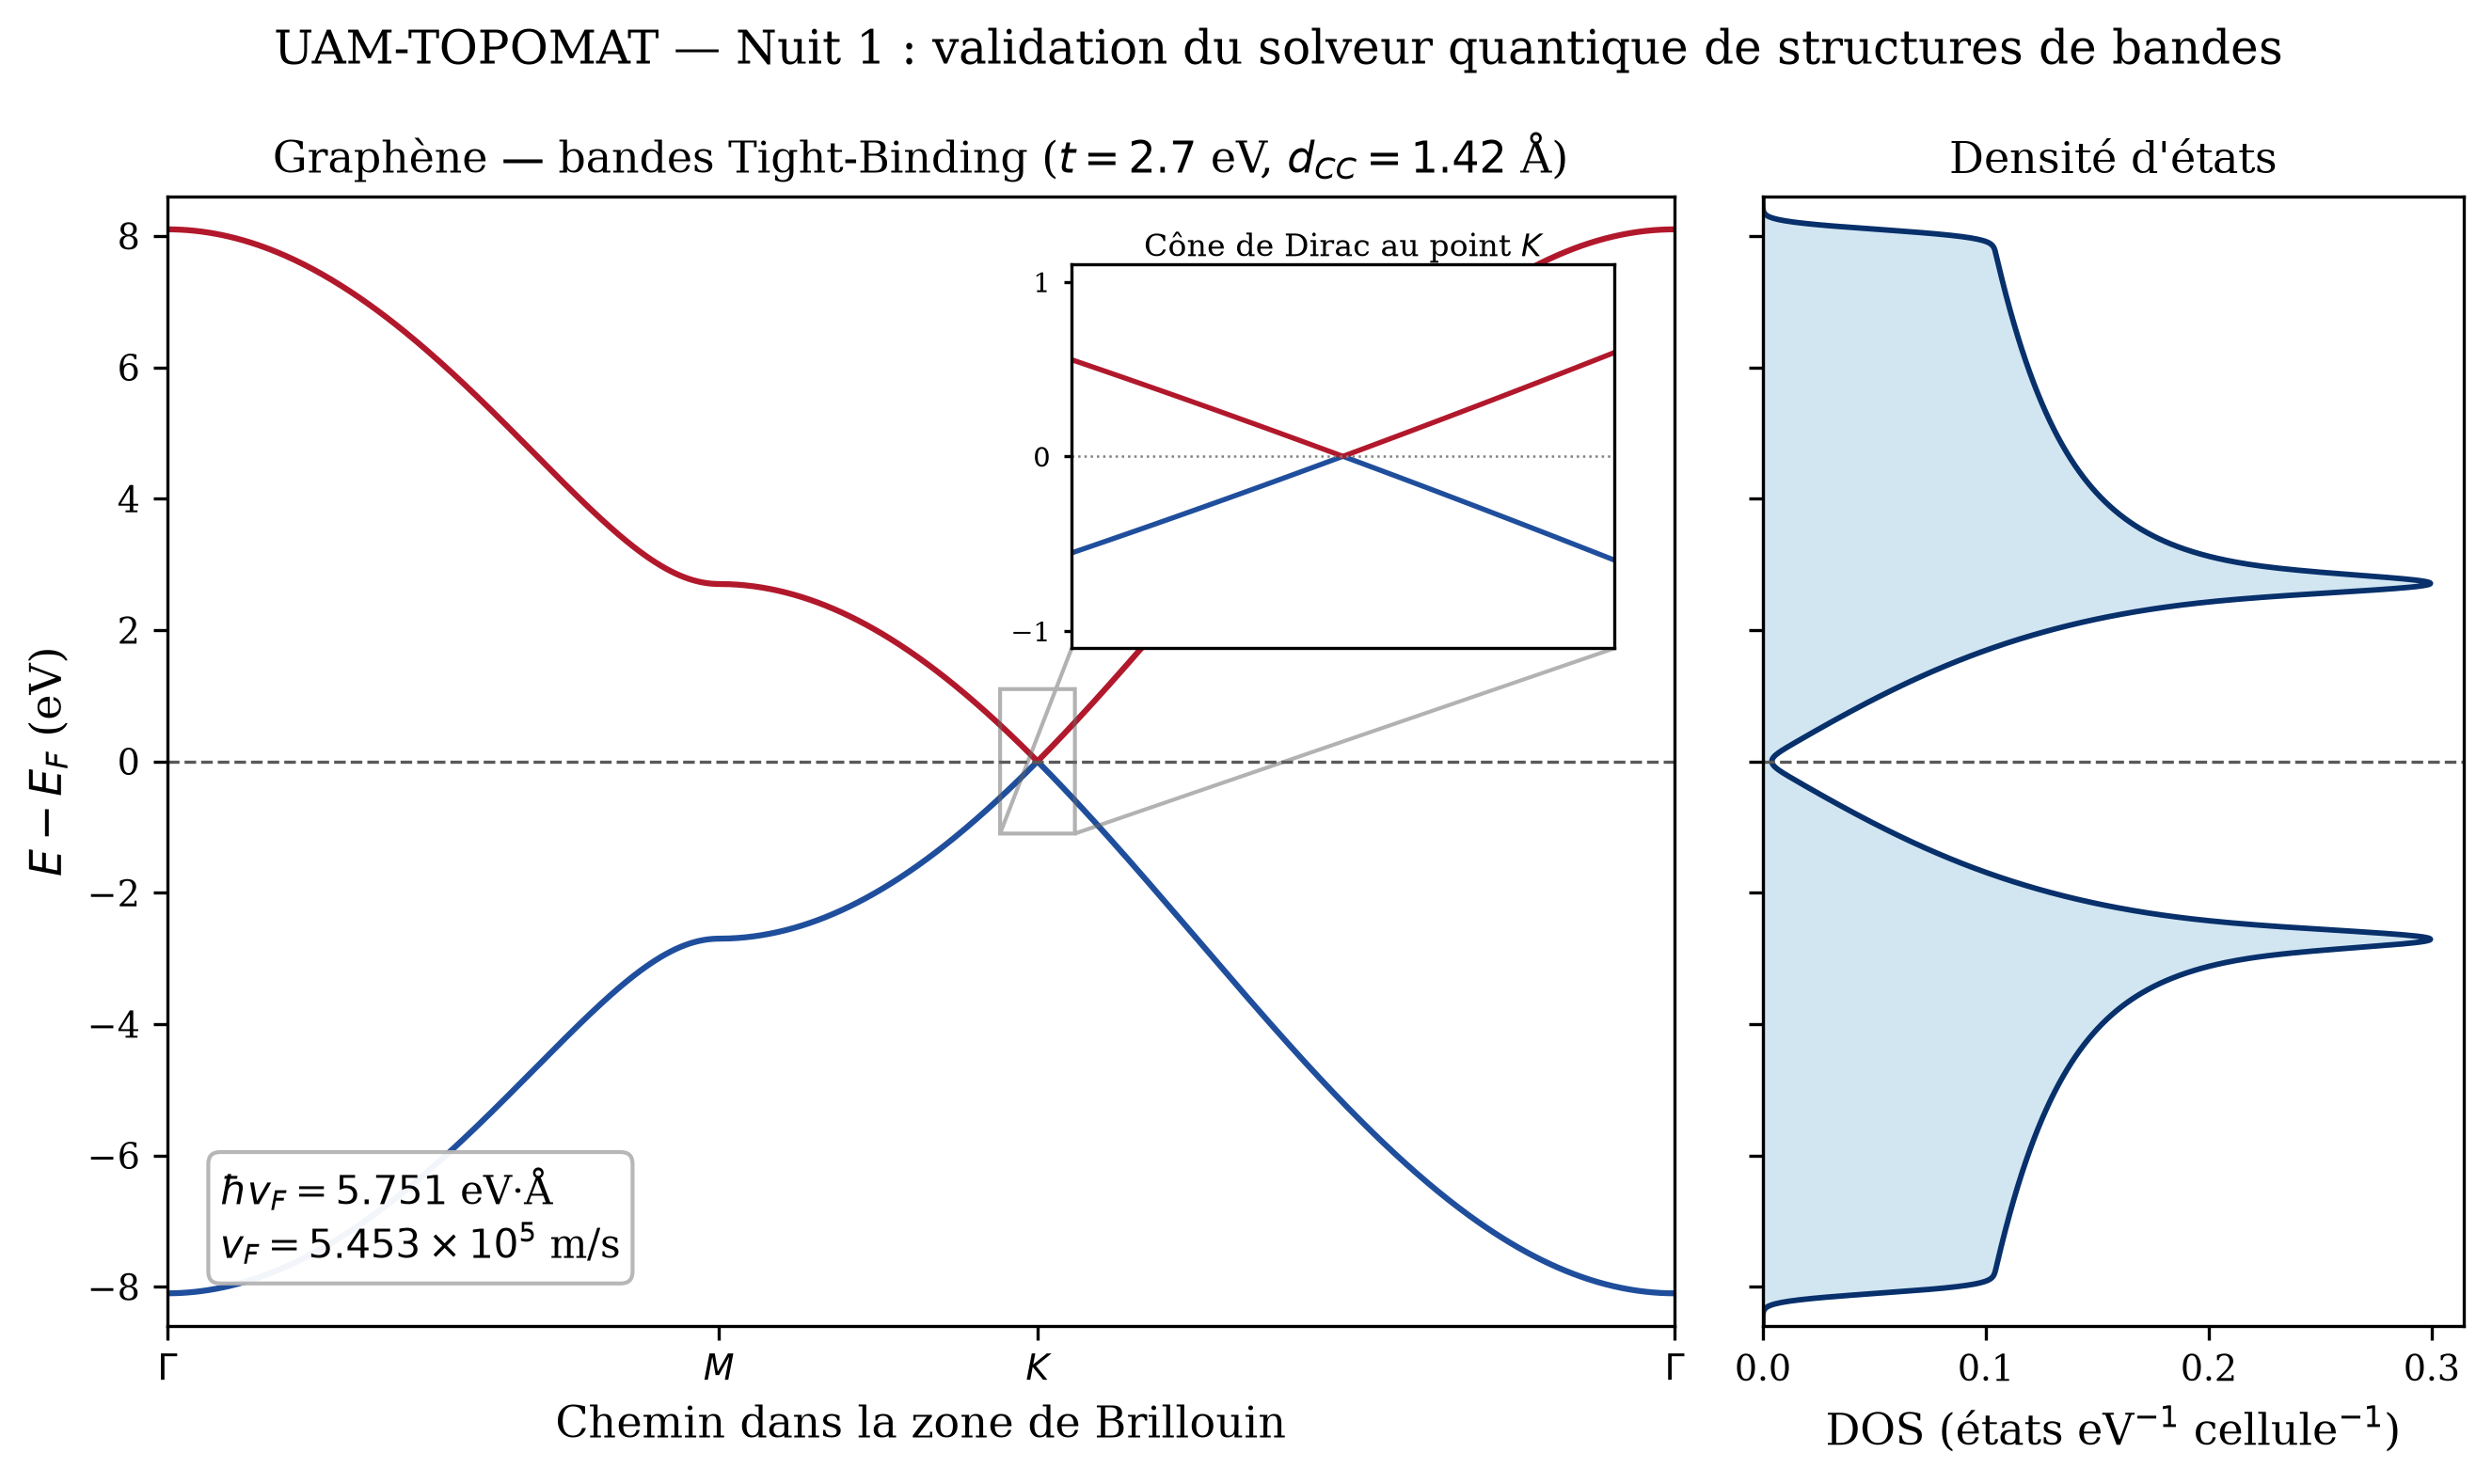
\includegraphics[width=\linewidth]{night1_bands_dos.png}
\caption{Structure de bandes Tight-Binding et densité d'états du graphène —
validation Nuit 1 du projet \TOPOMAT. Figure produite à 300~dpi par
\texttt{tests/test\_night1.py}.}
\label{fig:night1}
\end{figure}

\section{Conclusion et perspectives}
Le solveur quantique et le moteur cristallographique sont opérationnels et
validés. Les nuits suivantes étendront le formalisme aux invariants
topologiques (Berry, Chern), à la réponse optique et aux fonctions
thermodynamiques des pérovskites et MXènes sahéliens.

\end{document}
